\documentclass{beamer}

\usetheme{Boadilla}
\useinnertheme{rectangles}
\useoutertheme{infolines}
%\usecolortheme{dolphin}

\title[Tool Interoperability in MFE]{
  Tool Interoperability in \\ the Maude Formal Environment
}

\author[Dur\'an, Rocha, \'Alvarez]{
  Francisco Dur\'an\inst{1} \and Camilo Rocha\inst{2} \and Jos\'{e} M. \'Alvarez\inst{1}
}

\institute[UMA, U of I]{
  \inst{1}Universidad de M\'alaga \\
  \inst{2}University of Illinois at Urbana-Champaign
}

\date[Calco-Tools 2011]{
  \\
  4th Conference on Algebra and Coalgebra in Computer Science \\
  August 31, 2011 \\
  Winchester, UK
}


\newcommand{\csuea}[2]{{\rm CSU}_{#2}(#1)}
\newcommand{\vind}{\vdash_{\rm ind}}
\newcommand{\rcal}{\mathcal{R}}
\newcommand{\kcal}{\mathcal{K}}
\newcommand{\mcal}{\mathcal{M}}
\newcommand{\tcal}{\mathcal{T}}
\newcommand{\acal}{\mathcal{A}}
\newcommand{\ecal}{\mathcal{E}}
\newcommand{\ecalpi}{\mathcal{E}_\Pi}
\newcommand{\reach}{{\rm reach}}
\newcommand{\states}{\mathfrak{s}}
\newcommand{\iffo}{\Longleftrightarrow}
\newcommand{\mimps}{\Longrightarrow}
\newcommand{\imps}{\Rightarrow}
\newcommand{\rews}{\rightarrow}
\newcommand{\rewsn}[1]{\stackrel{#1}{\rews}}
\newcommand{\true}{\top}
\newcommand{\false}{\bot}
\newcommand{\eq}[2]{#1 = #2}
\newcommand{\ceq}[3]{#1 = #2 \; {\rm if} \; #3}
\newcommand{\qeq}[3]{(\forall #1) \; #2 = #3}
\newcommand{\qceq}[4]{(\forall #1) \; #2 = #3 \; {\rm if} \; #4}
\newcommand{\rl}[2]{#1 \rews #2}
\newcommand{\crl}[3]{#1 \rews #2 \; {\rm if} \; #3}
\newcommand{\qrl}[3]{(\forall #1) \; #2 \rews #3}
\newcommand{\qcrl}[4]{(\forall #1) \; #2 \rews #3 \; {\rm if} \; #4}
\newcommand{\qrln}[4]{(\forall #1) \; #2 \rewsn{#4} #3}
\newcommand{\qcrln}[5]{(\forall #1) \; #2 \rewsn{#5} #3 \; {\rm if} \; #4}

\begin{document}

\begin{frame}
  \titlepage
\end{frame}

\begin{frame}
  \frametitle{Main Contribution}

  The Maude Formal Environment (MFE) is an executable formal specification in Maude
  within which a user can interact with tools to mechanically verify properties
  of Maude specifications

  \begin{itemize}
    \item<2-> it has been designed to be easily extended with tools having
      heterogeneous designs

    \begin{itemize}
      \item<2-> it currently offers five tools
    \end{itemize}

    \item<3-> it implements a mechanism to keep track of pending proof
      obligations

    \item<4-> its tool interoperability allows for discharging proof obligations of
      different nature without switching between different tool environments
      and presents the user with a consistent user interface

    \item<5-> it allows the execution of several instances of each tool

  \end{itemize}
\end{frame}


\begin{frame}
  \frametitle{Motivation}
  \framesubtitle{The Example of Readers and Writers}

  We want to check in the {\tt R+W} system that it is never the case that
  more than (i) one writer or (ii) writers and readers share a critical 
  resource at the same time. A state is represented by a term
  \[\langle r,w\rangle\]
  where $r$ and $w$ are the number of readers and writers accessing the critical resource.

  \begin{itemize}
    \item<2-> {\tt R+W} needs to be executable, i.e., its equations ground
      Church-Rosser and terminating, and its rewrite rules ground coherent
      with respect the equations
    \item<3-> for initial state $\langle 0,0\rangle$, the set of initial states
      is infinite, so we apply a state abstraction in {\tt R+W-ABS} which
      needs to be checked executable
  \end{itemize}
\end{frame}

\begin{frame}
  \frametitle{Outline}
  \tableofcontents
\end{frame}

\section{Tools in the Environment}

\begin{frame}
  \frametitle{Outline}
  \tableofcontents[currentsection]
\end{frame}

\begin{frame}
  \frametitle{Tool Overview}

  In the current version of MFE one can interact with the following tools:

  \begin{description}
    \item[MTT]<2-> {\em Maude Termination Tool}
      
      termination of equational and rewrite specifications

    \item[SCC]<3-> {\em Sufficient Completeness Checker}
      
      sufficient completeness and freeness of equational specifications,
      and deadlock of rewrite specifications

    \item[CRC]<4-> {\em Church-Rosser Checker}
      
      ground confluence and sort-decreasingness of equational specifications

    \item[ChC]<5-> {\em Maude Coherence Checker}
      
      ground coherence of rewrite specifications

    \item[ITP]<6-> {\em Inductive Theorem Prover}
      
      inductive properties of equational specifications

  \end{description}
\end{frame}

\begin{frame}
  \frametitle{Tool-dependency Graph in MFE}

  One important aspect in the integration task is the interaction complexity due to the
  nontrivial dependencies among tools

  \begin{center}
    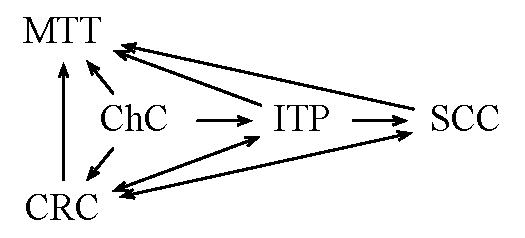
\includegraphics[width=6cm]{tool-dep}
  \end{center}
\end{frame}

\section{Design and Main Features}

\begin{frame}
  \frametitle{Outline}
  \tableofcontents[currentsection]
\end{frame}

\begin{frame}
  \frametitle{MFE Design Overview}

  \begin{itemize}
    \item MFE is modeled in Maude as an interactive object-based system where
      tools are objects, the communication mechanism is message passing, and
      user interaction is available through Full Maude
    \item[]
    \item<2-> integration and interoperation of tools within MFE is module-centric
      given that its main purpose is to support formal analysis of Maude modules
    \item[]
    \item<3-> although some classes and functionality are provided in MFE, it imposes
      no constraint on how each tool should model its particular domain or maintains
      its internal state
  \end{itemize}
\end{frame}

\begin{frame}
  \frametitle{Main Classes}

  The object-oriented model of MFE consists of three main classes

  \begin{description}
    \item[\texttt{  \small Proof}] class of proof objects that keep the state of specific proof requests
    \item[\texttt{  \small Tool}] class of tool objects that keep the life-cycle of proof objects
    \item[\texttt{  \small Controller}] inherits from Full Maude's {\tt DatabaseClass} and
      provides a centralized entry point for handling user request
  \end{description}
\end{frame}

\begin{frame}
  \frametitle{User Interaction}

  The user interacts with the environment via commands

  \begin{itemize}
    \item<2-> each command is encapsulated as a message in the object configuration
    \item<3-> each tool object and the controller object have a module defining the
      signature of commands it can handle
    \begin{itemize}
      \item the controller handles any command it can parse
      \item if the controller receives a command it cannot parse, then it delegates
        the message to the {\em active} tool
      \item if the tool can parse the delegated command, then it notifies the controller
        and handles the command
      \item otherwise, it will notify the failure to the controller, which in turn
        will output an error message to the user
    \end{itemize}
  \end{itemize}
\end{frame}

\begin{frame}
  \frametitle{Commands in MFE}
  
  MFE provides the following user commands:

  \begin{description}
    \item[\texttt{  \small(select tool <tool-name> .)}]
      %\noindent \texttt{  \small(select tool <tool-name> .)} 
      sets \texttt{\small<tool-name>} as the {\em active} tool
    \item[\texttt{  \small(MFE help .)}] 
      %\noindent \texttt{  \small(MFE help .)}  
      shows MFE's help information
    \item[\texttt{  \small(show global state .)}] 
      %\noindent \texttt{  \small(show global state .)}  
      shows the state of the environment
  \end{description}

  \vspace{0.2cm}

  \pause
  
  The tools available in MFE's current release provide at least the following
  commands:

  \begin{description}
    \item[\texttt{  \small(<tool-name> help .)}]
      %\noindent \texttt{  \small(<tool-name> help .)}
      shows the help information of tool \texttt{\small<tool-name>}
      %information on the commands available in the active tool.
    \item[\texttt{  \small(show state .)}]
      %\noindent \texttt{  \small(show state .)}
      shows the state of the tool
  \end{description}
\end{frame}

\begin{frame}
  \frametitle{Proof Obligations}

A tool in MFE keeps track of both its pending and discharged proof obligations

\begin{itemize}
  \item<2-> a user can submit proof obligations to other tools by means of the following
    command and then be notified when these are discharged

  \begin{description}
    \item[\texttt{  (submit .)}]
  \end{description}

  \item<3-> when all proof obligations
    in the verification task of a module's property are discharged, 
    the corresponding tool notifies 
    the success result to the user or to the tool originating the verification task

\end{itemize}

\end{frame}


\begin{frame}
  \frametitle{Trusting Proof Obligations}

  Tools in general can impose constraints on its inputs

  \begin{itemize}
    \item<2-> for instance,
      SCC does not support parametric modules but proofs for 
      such modules could be obtained by hand or using another tool

    \item<3-> MFE offers the following command for keeping track of 
      proofs obtained outside the environment

    \begin{description}
      \item[\texttt{  (trust .)}]
    \end{description}
  \end{itemize}
\end{frame}

\begin{frame}
  \frametitle{External Utilities}

  For tools which depend on external
  utilities not directly available from Maude such as MTT and SCC, 
  we have extended the latest release of the Maude system
  with {\em built-in} operators associated with appropriate
  C++ code that interacts with the external tools
\end{frame}

\section{Demo}

\begin{frame}
  \frametitle{Outline}
  \tableofcontents[currentsection]
\end{frame}

\begin{frame}
  \frametitle{Obtaining and Using MFE}

    The tool, the pimped version of Maude, 
    and more examples are available at 
    \begin{center}
      \textcolor{blue}{\url{http://maude.lcc.uma.es/MFE}}
    \end{center}
    \begin{flushright}
      Thank you!
    \end{flushright}
\end{frame}

\end{document}
